\chapter{Communication Strategies}

This thesis evaluates and compares several communication strategies for Sparse Matrix-Vector Multiplication (SpMV) in a parallel, distributed memory setting. During each iteration of SpMV, every process computes a partial result of the output vector 
\(y\).
\medskip

In subsequent iterations, these computed values may be required by other processes to proceed with their own calculations. To ensure correctness, it is therefore necessary to communicate between processes so that each has access to the values it depends on. This section outlines a progression of increasingly efficient strategies for managing this communication.

\section{1a - Exchange entire vector}

The most straightforward approach is to have each rank send all of its computed values of 
\(y\) to every other rank. This ensures that all processes possess a complete and updated copy of the output vector before the next iteration. This strategy can be implemented using MPI’s collective communication operation \texttt{MPI\_Allgatherv}, which accommodates variable message sizes from each rank. Figure \ref{fig:1acomm} illustrates the state of the \(y\) vector before and after communication using this strategy.


% The most basic communication strategy involves sending all values of \(y\) computed by each rank, to every other rank. This communication strategy results in each rank having all newly computed values of \(y\). In order to achieve this, we use MPI's \textit{allgather} fucntion, or more specifically we use \texttt{MPI\_Allgatherv}, which allows for each rank sending a different amount of values to other ranks. Figure \ref{fig:1acomm} illustrates the \(y\) vector before and after communication takes place. 

\begin{figure}[H]
    \centering
    \begin{subfigure}[t]{0.45\textwidth}
        \centering
        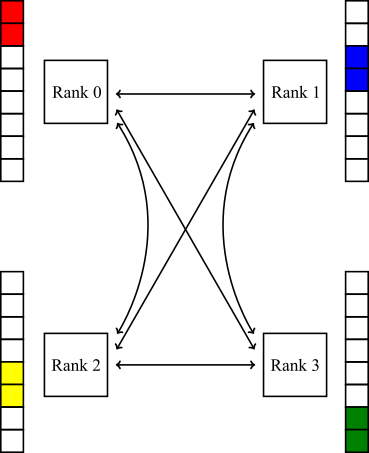
\includegraphics[width=\linewidth]{1acomm.png}
        \caption{\(y\) before communication.}
        \label{fig:1acomm1}
    \end{subfigure}
    \hfill
    \begin{subfigure}[t]{0.45\textwidth}
        \centering
        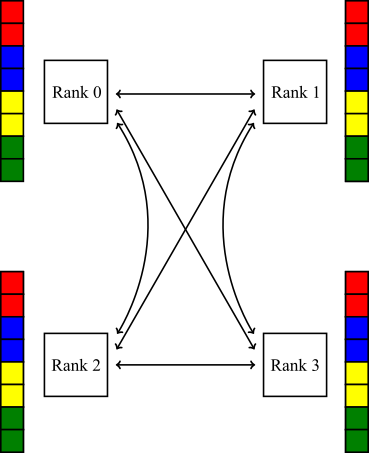
\includegraphics[width=\linewidth]{1acommdone.png}
        \caption{\(y\) after communication.}
        \label{fig:1acomm2}
    \end{subfigure}
    \caption{Visual representation of the \(y\) vector in communication strategy 1a.}
    \label{fig:1acomm}
\end{figure}

\begin{algorithm}[H]
    \caption{1a - Exchange entire vector}
    \SetAlgoVlined
    % \SetKwInOut{Input}{Input}
    % \SetKwInOut{Output}{Output}
    % \Input{}
    % \Output{\newline}

    \For{each iteration}{
        spmv(g,x,y)\\
        MPI\_Allgatherv(local\_y, sendcount, MPI\_DOUBLE, y, recvcounts, displs, MPI\_DOUBLE, MPI\_COMM\_WORLD)\\
        swap pointers of \(x\) and \(y\)

    }

\end{algorithm}

\section{1b - Exchange only separators}

An improvement to the previous strategy can be achieved by recognizing that only separator values—those required by multiple processes—must be communicated. Non-separator values are used exclusively by the process that computed them and therefore do not need to be communicated.

To facilitate this strategy, separator values are reordered such that they appear at the beginning of each process's local segment of \(y\). Once this structure is established, communication is performed using \texttt{MPI\_Allgatherv}, transmitting only the subset of \(y\) that contains separator values. The number of separators on each process must be known beforehand, which can be computed by counting the number of elements that have neighbours belonging to a different partition.


\subsection{Reordering}
After partitioning the matrix into different parts, we obtain a partition vector \(p\), where the \(p[i]\) stores the index of the partition the \(i^{\text{th}}\) entry in \(A_{p}\). It is necessary to reorder the entries in \(A_{p}\) in accordance with the partition vector, such that all entries belonging to the same partition are stored in sequence. The algorithm below gives an outline of how this can be achieved. Here \(n_{p}\) is the number of partitions, \(n_{r}\) is the size of \(A_{p}\), and \(n_{c}\) is the size of \(A_{j}\) and \(A_{x}\).

\begin{algorithm}[H]
    \caption{Reordering of Separators}
    \SetAlgoVlined
    \SetKwInOut{Input}{Input}
    \SetKwInOut{Output}{Output}
    \Input{\(n_{p}, n_{r}, n_{c}, p, A_{p}, A_{j}, A_{x}\)}
    \Output{Reordered \(A_{p}, A_{j}, A_{x}\)}
    
    newId \(\gets [0] \cdot n_{r}\)\\
    oldId \(\gets [0] \cdot n_{r}\)\\
    id \(\gets 0\)\\
    \(p_{0} \gets 0\)\\
    \phantom{a}\\
    
    \For{\(r \in \{0, \dotsc, n_{p}-1\}\)}{
        \For{\(i \in \{0, \dotsc, n_{r}-1\}\)}{
            \If{\(p[i] = r\)}{
                oldId[id] \(\gets i\)\\
                newId[i] \(\gets\) id\\
                id \(\gets\) id + 1\\
            }
        }
        \(p[r+1] \gets\) id\\
    }
    \phantom{a}\\
    
    newV \(\gets [0] \cdot (n_{r} + 1)\)\\
    newE \(\gets [0] \cdot n_{c}\)\\
    newA \(\gets [0] \cdot n_{c}\)\\
    
    \phantom{a}\\
    \For{\(i \in \{0, \dotsc, n_{r}-1\}\)}{
        degree \(\gets A_{p}[\text{oldId}[i]+1] - A_{p}[\text{oldId}[i]]\)\\
        newV[\(i+1\)] \(\gets\) newV[i] + degree\\
    }
    \phantom{a}\\
    
    \For{\(i \in \{0, \dotsc, n_{r}-1\}\)}{
        degree \(\gets A_{p}[\text{oldId}[i]+1] - A_{p}[\text{oldId}[i]]\)\\
        \For{\(j \in \{0, \dotsc, \text{degree}-1\}\)}{
            newE[newV[i]+j] \(\gets A_{j}[A_{p}[\text{oldId}[i]] + j]\)\\
            newA[newV[i]+j] \(\gets A_{x}[A_{p}[\text{oldId}[i]] + j]\)\\
        }
        \For{\(j \in \{newV[i], \dotsc, newV[i+1]-1\}\)}{
            newE[j] \(\gets\) \text{newId}[newE[j]]\\
        }
    }
    \phantom{a}\\
    
    Overwrite \(A_{p} \gets\) newV, \(A_{j} \gets\) newE, \(A_{x} \gets\) newA\\
\end{algorithm}
% It becomes evident that this is a better strategy when we realize that it is not necessary to communicate non-separator values of \(y\), as these values are only ever needed by the rank they are computed on. Separators on the other hand, are needed by other ranks, and therefore need to be communicated. This strategy can be implemented by reordering and counting the number of separators on each rank, and only sending these values to all other ranks, again using \textit{allgather}.


\begin{figure}[H]
    \centering
    \begin{subfigure}[t]{0.45\textwidth}
        \centering
        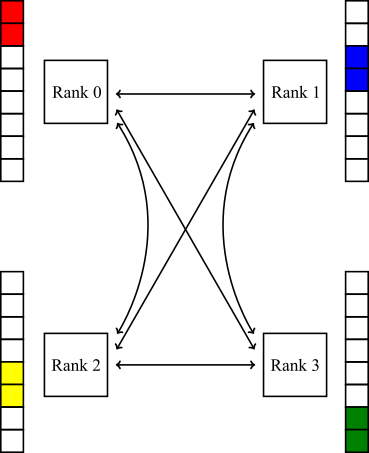
\includegraphics[width=\linewidth]{1acomm.png}
        \caption{Caption for image 1}
        \label{fig:1bcomm1}
    \end{subfigure}
    \hfill
    \begin{subfigure}[t]{0.45\textwidth}
        \centering
        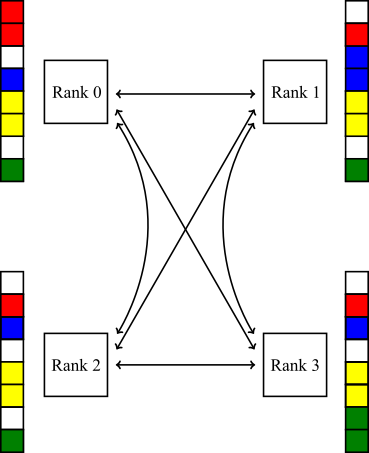
\includegraphics[width=\linewidth]{1bcommdone.png}
        \caption{Caption for image 2}
        \label{fig:1bcomm2}
    \end{subfigure}
    \caption{Main figure caption describing both subfigures}
    \label{fig:1bcomm}
\end{figure}


\section{1c - Exchange only required separators}
Further reduciton to the communication volume can be achieved by observing that not all separator values are required by every process. As the number of partitions increases, the set of dependencies between partitions tends towards sparcity. As a consequence of this, certain sets of separators may only need to be communicated to a given subset of processes. Using this strategy, each process only communicates its set of separator values to the processes that require them.
% Another observation that can be made in order to further reduce the communication load comes when we realize that not every rank necessarily needs every separator. As we increase the number of partitions in the matrix, we increase the chance that there exists ranks whose separators are disjoint. If this is the case, we can further reduce the communication load by only sending a ranks separator to another rank if it is necessary 


% Not all ranks need all separators. If rank 0 has some number of separators, none of which are needed by say rank 2, we don't need to communicate them. This strategy further reduces the communication load.

\begin{figure}[H]
    \centering
    \begin{subfigure}[t]{0.45\textwidth}
        \centering
        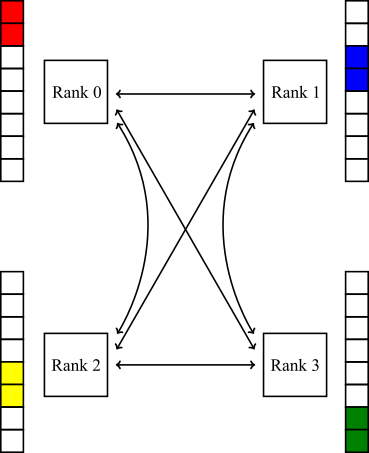
\includegraphics[width=\linewidth]{1acomm.png}
        \caption{Caption for image 1}
        \label{fig:1ccomm1}
    \end{subfigure}
    \hfill
    \begin{subfigure}[t]{0.45\textwidth}
        \centering
        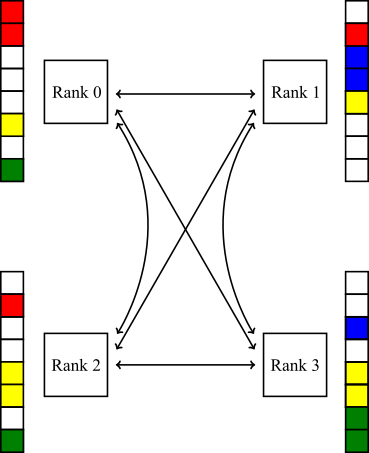
\includegraphics[width=\linewidth]{1ccommdone.png}
        \caption{Caption for image 2}
        \label{fig:1ccomm2}
    \end{subfigure}
    \caption{Main figure caption describing both subfigures}
    \label{fig:1ccomm}
\end{figure}

\section{1d - Exchange only required separator values}
The final strategy aims to minimize communication overhead by transmitting only the exact subset of separator values that are both computed by and required for inter-process computation. If a specific separator value computed by one process is needed by exactly one other process, then only that single recipient receives the value.

This approach eliminates all unnecessary data transfers but introduces additional complexity in managing communication schedules. Dependencies must be mapped at a fine-grained level, and communication patterns must be explicitly tailored to the structure of the matrix and its partitioning.
